\documentclass[12pt,compress,aspectratio=169]{beamer}

\mode<presentation>
{
  \usetheme{Singapore}
  \setbeamersize{text margin left=.5cm,text margin right=.5cm}
%  \setbeamertemplate{navigation symbols}{} % suppress nav bar
%  \setbeamercovered{transparent}
}
\usefonttheme{professionalfonts}
\usepackage{amsmath}
\usepackage{graphicx}
\usepackage{tikz}
\usepackage{mathpazo}
\usepackage[scaled]{helvet}
\usepackage{xcolor,colortbl}
\usepackage{hyperref}
\usepackage{siunitx}

\sisetup{
  number-math-rm=\mathnormal,
  per-mode=symbol
}


\title{Topic 2: Dynamics}
\subtitle{Advanced Placement Physics}
\author[TML]{Dr.\ Timothy Leung}
\institute{Olympiads School}
\date{Summer 2018}

\newcommand{\pic}[2]{\includegraphics[width=#1\textwidth]{#2}}
\newcommand{\mb}[1]{\ensuremath\mathbf{#1}}
\newcommand{\magdir}[2]{#1\textrm{ [#2]}}
\newcommand{\eq}[2]{\vspace{#1}{\Large\begin{displaymath}#2\end{displaymath}}}

\begin{document}

\section{Dynamics}

\begin{frame}
  \frametitle{Dynamics}
  While we use \textbf{kinematics} to describe the motion of any object
  mathematically, we use \textbf{dynamics} to describe \emph{what} causes
  motion.
  \begin{itemize}
  \item Newton's three laws of motion
  \end{itemize}
\end{frame}



\subsection{Newton's Laws}

\begin{frame}
  \frametitle{Newton's First Law}
  \begin{center}
    \fbox{
      \begin{minipage}{.8\textwidth}
        \textbf{An object at rest or in uniform motion will remain at rest or
          in uniform motion unless acted on by a net external force.}
      \end{minipage}
    }
  \end{center}

  \vspace{.3in}
  \begin{itemize}
  \item Uniform motion: constant velocity
  \item Keep in mind that an object at rest is also in uniform motion: it has
    a velocity of zero.
  \item Common Examples:
    \begin{itemize}
    \item spacecraft in ``deep space''
    \item hockey puck sliding on very smooth ice
    \end{itemize}
  \end{itemize}
\end{frame}


\begin{frame}
  \frametitle{Newton's Second Law}
  \begin{center}
    \fbox{
      \begin{minipage}{.8\textwidth}
        \textbf{The sum of the forces acting on an object is proportional to
          its mass and its acceleration}.
      \end{minipage}
    }
  \end{center}

  \eq{-.2in}{
    \boxed{\mb{F}_{\textrm{net}}=\Sigma\mb{F}=m\mb{a}}
  }
  
  \begin{center}
    \begin{tabular}{l|c|l}
      \rowcolor{pink}
      \textbf{Quantity} & \textbf{Symbol} & \textbf{SI Unit} \\ \hline
      Net force (sum of all forces)  & $\mb{F}_{\textrm{net}}$ & \si{N}\\
      Mass         & $m$       & \si{kg}\\
      Acceleration & $\mb{a}$  & \si{m/s^2}\\
    \end{tabular}
  \end{center}

  Actually, this equation isn't exactly what Newton wrote. He wrote that force
  is the rate of change of the ``quantity of motion'' (momentum). We will be
  looking into that more next class.
\end{frame}


\begin{frame}
  \frametitle{Newton's Third Law}

  \begin{center}
    \fbox{
      \begin{minipage}{.8\textwidth}
        \textbf{For every action there is an equal and opposite reaction.}
      \end{minipage}
    }
  \end{center}
 
  For every action force on an object (B) due to another object (A), there is a
  reaction force which is equal in magnitude but opposite in direction, on
  object (A), due to object (B):

  \eq{-.2in}{
    \boxed{\mb{F}_{\textrm{A on B}} = -\mb{F}_{\textrm{B on A}}}
  }
  
  The reaction forces act on different objects!
\end{frame}


\begin{frame}
  \frametitle{Example Problem}
  \framesubtitle{A Blast From the Past}
  This problem can get you started to remember how to do these problems, but it
  is a bit too easy for AP Physics.
  
  \vspace{.2in}\textbf{Example 1:} In old-style television picture tubes and
  computer monitors (cathode ray tubes), light is produced when fast-moving
  electrons collide with phosphor molecules on the surface of the screen. The
  electrons (mass $m=\SI{9.1e-31}{kg}$) are accelerated from rest in the
  electron ``gun'' at the back of the vacuum tube. Find the velocity of an
  electron when it exits the gun after experiencing an electric force of
  \SI{5.8e-15}{N} over a distance of \SI{3.5}{mm}.
\end{frame}



\begin{frame}{Forces}
  \begin{itemize}
  \item A \textbf{force} is the interaction between the objects.
    \begin{itemize}
    \item When there is interaction, then forces are created
    \item A ``push'' or a ``pull''
%    \item Gravity: interaction between to objects with mass
%    \item Electric force: interaction between two charged object
%    \item Nuclear force: interaction between protons, electrons and neutrons
    \end{itemize}

  \item Newton considered all forces acting at a single point of an object
    called the centre of gravity (``CG'')
    \begin{itemize}
    \item The centre of gravity is also called the center of mass (``CM'')
    \item If the density of an object is constant, then the CG is also the
      geometric centre (centroid) of the object
    \item Sooner we will look into how to find the center of mass of diferent
      things
    \end{itemize}
  \end{itemize}
\end{frame}



\begin{frame}{Forces}
  \begin{itemize}
  \item There are two broad categories of forces:
    \begin{itemize}
    \item\textbf{Contact forces} act between two objects that are in contact
      with one another
    \item\textbf{Non-contact forces} act between two objects without them
      touching each other. They are also called ``action-at-a-distance'' force
    \end{itemize}
    
  \item If the net force on an object is zero ($\Sigma\mb{F}=\mb{0}$) then the
    object is in a \emph{state of equilibrium}
    \begin{itemize}
    \item Dynamic equilibrium: the object is moving relative to us
    \item Static equilibrium: the object is not moving relative to us
    \end{itemize}  
  \end{itemize}
\end{frame}



\begin{frame}{Common Forces}
  Common everyday forces that we encounter in Physics 12 include:
  \begin{itemize}
  \item Gravitational force (weight) $\mb{F}_g$
  \item Normal force $\mb{F}_N$
  \item Friction (static $\mb{F}_s$ and kinetic $\mb{F}_k$)
  \item Tension $\mb{F}_T$
  \item Applied force $\mb{F}_a$
  \item Spring force $\mb{F}_e$
  \item Air resistance (drag) $\mb{D}$
  \item Electrostatic force $\mb{F}_q$ (E \& M exam)
  \item Magnetic force $\mb{F}_M$ (E \& M exam)
  \end{itemize}
\end{frame}



\begin{frame}{Gravity}
  \begin{itemize}
  \item The force of attraction between all objects with mass
    
    \eq{-.2in}{
      \boxed{\mb{F}_g=m\mb{g}}
    }
  \item Near surface of Earth, use $g=\SI{9.81}{m/s^2}$ or $g=\SI{10}{m/s^2}$
  \item There may be problems where you are asked to find the value of $g$ on
    some ``distant unknown planet''.
  \item $\mb{F}_g$ always points \textbf{down}
  \item Newton's law of universal gravity:

    \eq{-.3in}{
      \boxed{F_g=\frac{Gm_1m_2}{r^2}}\quad
      \text{\normalsize where}\quad
      G=\SI{6.67e-11}{m^3/kg.s^2}
    }
  \end{itemize}    
\end{frame}



\begin{frame}
  \frametitle{Friction}
  \begin{itemize}
  \item A force that opposes the sliding of two surface across one another
  \item Always act in a the direction opposite to motion or attempted motion
  \item Two types: \emph{static friction} and \emph{kinetic friction}
%  \item Proportional to how much force the two surfaces are pressed against
%    each other (expressed by normal force $F_N$)
%  \item Also depends on the type of surfaces--coefficient of friction
%    ($\mu_s$ for static, $\mu_k$ for kinetic), which depends on
%    \begin{itemize}
%    \item What materials the surfaces are made of
%    \item Whether a lubricant is used
%    \end{itemize}
  \end{itemize}
  
  \begin{center}
   \pic{.7}{graphics/friction.jpg}
  \end{center}
\end{frame}


\begin{frame}
  \frametitle{Static Friction}
  \begin{itemize}
  \item The friction between the two surfaces when there is no relative
    motion between them
  \item Static friction increases with increasing applied force
    $F_\mathrm{a}$. It is at maximum when the object is just about to move.
  \end{itemize}

  \eq{-.3in}{\boxed{\max F_s = \mu_sF_N}}

  \begin{itemize}
  \item $\mu_s$ is the static friction coefficient (does not have a unit)
  \item $F_N$ is the normal force
  \item I didn't use vector notation. This equation deals with the magnitude
    only
  \end{itemize}
  {\footnotesize (\textbf{Pro tip:} The symbol for the coefficient of friction
    $\mu$ is the Greek letter \emph{mu})}
\end{frame}

\begin{frame}
  \frametitle{Kinetic Friction}
  
  \eq{0pt}{\boxed{F_k = \mu_kF_N}}

  \begin{itemize}
  \item The friction between two surfaces moving relative to each other
  \item $F_k$ is constant along the path of movement as long
    as the normal force stays constant
  \item $\mu_k$ is the kinetic friction coefficient (does not have a unit). It
  is always lower than the static coefficient, otherwise nothing will ever move
    
    \eq{-.3in}{\mu_k\leq\mu_s}
  \end{itemize}
\end{frame}

\begin{frame}
  \frametitle{Normal Force}
  \begin{columns}
    \column{.25\textwidth}
    \begin{center}
    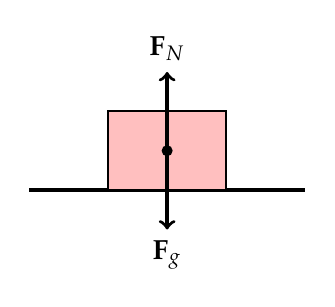
\begin{tikzpicture}{scale=1.5}
      \draw [very thick] (-1,0)--(2.5,0);
      \draw [fill=pink,thick] (0,0) rectangle (1.5,1);
      \fill (.75,.5) circle(2pt);
      \draw [->,very thick] (.75,.5)--(.75,-.5)
      node[pos=1,below]{$\mb{F}_g$};
      \draw [->,very thick] (.75,.5)--(.75,1.5)
      node[pos=1,above]{$\mb{F}_N$};
    \end{tikzpicture}
    \end{center}
    \begin{displaymath}
      \mb{F}_g=m\mb{g}=-\mb{F}_N
    \end{displaymath}
    
    \column{.75\textwidth}
    \begin{itemize}
    \item A force a surface exerts on another object that it is in contact with
    \item Always \textbf{perpendicular} to the contact surface
    \item\textbf{Special case:} When an object is on a horizontal surface
      with no additional applied force, the magnitude of the normal force is
      equal to the magnitude of the weight of the object, i.e.\ $F_N=F_g$
    \end{itemize}
  \end{columns}
\end{frame}

\begin{frame}
  \frametitle{Normal Forces on a Slope}
  For this case, we label the $x$-axis to be along the slope, and $y$-axis to
  be perpendicular to the slope.
  \begin{columns}
    \column{.35\textwidth}
    \begin{center}
      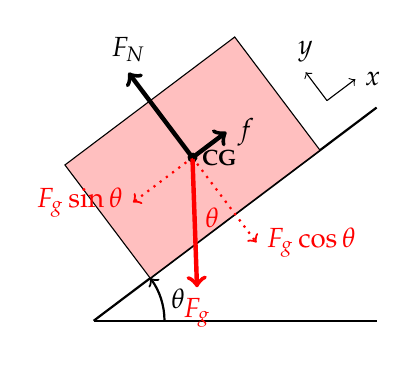
\begin{tikzpicture}[scale=.9]
        \draw[thick] (-1,0)--(3,0);
        \draw[thick,->](0,0) arc(0:37:1) node[midway,right] {$\theta$};
        \begin{scope}[rotate around={37:(-1,0)}]
          \draw[->](3.5,.5)--(4,.5) node[pos=1,right]{$x$};
          \draw[->](3.5,.5)--(3.5,1) node[pos=1,above]{$y$};
          \draw[thick] (-1,0)--(4,0);
          \draw[fill=pink] (0,0) rectangle (3,2);
          \fill(1.5,1) circle (2pt) node[right]{\footnotesize\textbf{CG}};
          \draw [->,thick,dotted,red] (1.5,1)--(1.5,-.5)
          node[pos=1,right]{$F_g\cos\theta$};
          \draw [->,thick,dotted,red] (1.5,1)--(.45,1)
          node[pos=1,left]{$F_g\sin\theta$};
          \draw [->,ultra thick,red] (1.5,1)--(.45,-.5)
          node[pos=1,below]{$F_g$}
          node[pos=.3,below right]{$\theta$};
        \draw [->,ultra thick] (1.5,1)--(1.5,2.5) node[pos=1,above]{$F_N$};
        \draw [->,ultra thick] (1.5,1)--(2.1,1) node[pos=1,right]{$f$};
        \end{scope}
      \end{tikzpicture}
    \end{center}
    
    \column{.65\textwidth}
    \begin{itemize}
    \item If on a slope: $F_N=F_g\cos\theta$
      \begin{itemize}
      \item $F_N$ decreases as ramp angle $\theta$ increases
      \item Obviously, at $\theta=\ang{90}$, $F_N=0$!
      \end{itemize}
    \item $F_g$ has a component along the ramp $F_g\sin\theta$ that
      wants to slide the block down.
    \item Friction force $f$ opposes the motion
      \begin{itemize}
      \item Be careful: if the block is moving \emph{up} the ramp with an
        applied force, then $f$ will point \emph{down} the ramp
      \end{itemize}
    \end{itemize}
  \end{columns}
\end{frame}

\begin{frame}
  \frametitle{Example Problem}
  \textbf{Example 8:} To move a \SI{45}{kg} wooden crate across a wooden floor
  ($\mu=0.20$), you tie a rope onto the crate and pull on the rope. While you
  are pulling the rope with a force of \SI{115}{N}, it makes an angle of
  \ang{15}
  with the horizontal. How much time elapses between the time at which the
  crate just starts to move and the time at which you are pulling it with a
  velocity of \SI{1.4}{m/s}?
  \begin{center}
    \pic{.5}{graphics/pull-box.png}
  \end{center}
\end{frame}

\begin{frame}
  \frametitle{Example Problem}
  \textbf{Example 9:} You are holding an \SI{85}{kg} trunk at the top of a ramp
  that slopes from a moving van to the ground, making an angle of \ang{35} with
  the ground. You lose your grip and the trunk begins to slide.
  \begin{itemize}
  \item If the coefficient of friction between the trunk and the ramp is
    $0.42$, what is the acceleration of the trunk?
  \item If the trunk slides \SI{1.3}{m} before reaching the bottom of the ramp,
    for what time interval did it slide?
  \end{itemize}
\end{frame}

\begin{frame}
  \frametitle{Example: Vertical Motion}
  \textbf{Example 10:} A \SI{55}{kg} person is standing on a scale in an
  elevator. If
  the scale is calibrated in \emph{newtons}, what is the reading on the scale
  when the elevator is not moving? If the elevator begins to accelerate upward
  at \SI{.75}{m/s^2}, what will be the reading on the scale?
\end{frame}


\subsection{Connected Bodies}


\begin{frame}
  \frametitle{Tension in a Cable}
  \textbf{Tension:} The magnitude of the force exerted on and by a cable, rope,
  or string. How do engineers determine the amount of tension needed for a
  specific object (bridges, floors or light fixtures)?

  \begin{itemize}
  \item You can't push on a rope
  \item Assume the cable/rope/string to be mass less
  \item Force can change direction when used with pulleys
  \end{itemize}
\end{frame}



\begin{frame}
  \frametitle{Example Problem}
  \textbf{Example 11:} An elevator filled with people has a total mass of
  \SI{2245}{kg}. As the elevator begins to rise, the acceleration is
  \SI{.55}{m/s^2}. What is the tension in the cable that is lifting the
  elevator?   
\end{frame}



\begin{frame}
  \frametitle{Applying Newton's Third Law on Connected Bodies}
  \begin{center}
    \pic{.7}{graphics/worldslongestroadtrainwithpowertrailer8.jpg}
  \end{center}
  \begin{itemize}
  \item Usually the objects are connected by a cable or a solid linkage with
    negligible mass
  \item All object have the same acceleration
  \item Require multiple free-body diagrams
  \end{itemize}
\end{frame}



\begin{frame}
  \frametitle{Solving Connected-Bodies Problems}
  To solve a connected-bodies problem, you can follow these procedures:
  \begin{enumerate}
  \item Draw a FBD on each of the objects
  \item Sum all the forces on all the objects along the direction of motion
    \begin{itemize}
    \item Direction of motion are usually very obvious
    \item All the tension forces should cancel, because they are ``internal''
      forces and not ``external forces''
    \end{itemize}
  \item Compute the acceleration of the entire system using Newton's second law
    \begin{itemize}
    \item Remember that every object has the same acceleration!
    \end{itemize}
  \item Go back to the FBD of each of the objects and compute the unknown
    forces (usually tension)
  \end{enumerate}
\end{frame}



\begin{frame}
  \frametitle{Connected Bodies: Example}
  \textbf{Example 12:} A tractor-trailer pulling two trailers starts from rest
  and accelerates to a speed of \SI{16.2}{km/h} in \SI{15}{s} on a straight,
  level
  section of highway. The mass of the truck itself (T) is \SI{5450}{kg}, the
  mass of the first trailer (A) is \SI{31500}{kg}, and the mass of the second
  trailer (B) is \SI{19600}{kg}.
  \begin{itemize}
  \item What magnitude of force must the truck generate in order to accelerate
    the entire vehicle?
  \item What magnitude of force must each of the trailer hitches withstand
    while the vehicle is accelerating?
  \end{itemize}
  For this problem we will assume that frictional forces are negligible in
  comparison with the forces needed to accelerate the large masses.
\end{frame}



%\begin{frame}
%  \frametitle{Example Problem: Towing}
%  \textbf{Example 7:} A $1700kg$ car is towing a larger vehicle with mass
%  $2400kg$. The two vehicles accelerate uniformly from a stoplight, reaching a
%  speed of $15km/h$ in $11s$. Find the force needed to accelerate the connected
%  vehicles, as well as the minimum strength of the rope between them.
%  \begin{center}
%    \pic{.55}{graphics/car-tow-truck.png}
%  \end{center}
%\end{frame}



\begin{frame}
  \frametitle{Example Problem: Atwood Machine}
  An \textbf{Atwood machine} is made of two objects connected by a rope that
  runs over a pulley. The pulley allows the direction of force and direction
  of motion to change between two objects.
  \begin{columns}
    \column{.5\textwidth}
    \begin{center}
      \pic{1}{graphics/atwood.png}
    \end{center}
    \column{.5\textwidth}
    \textbf{Example 13:} The object on the left ($m_1$) has a mass of
    \SI{8.5}{kg} and the object on the right ($m_2$) has a mass of \SI{17}{kg}.
    \begin{itemize}
    \item What is the acceleration of the masses?
    \item What is the tension in the rope?
    \end{itemize}
  \end{columns}
\end{frame}



\begin{frame}
  \frametitle{A More Typical Problem}
  \textbf{Example 14:}
  More typically, an Atwood machine problem is one where two objects are
  sliding on a surface. These surfaces may have (or may not) have friction.
  In this example, two blocks are connected by a mass-less string over a
  friction-less pulley as shown in the diagram.
  \begin{columns}
    \column{.45\textwidth}
    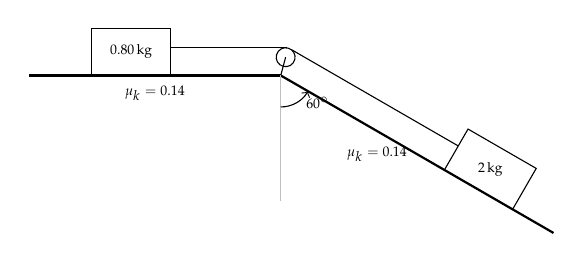
\begin{tikzpicture}[scale=.8]
      \draw[thick](0,0)--(-4,0) node[midway,below]{\tiny $\mu_k=0.14$};
      \draw(-1.75,0) rectangle(-3,.75) node[midway]{\tiny\SI{0.80}{\kg}};
      \draw(-1.75,.44)--(.1,.44);
      \begin{scope}[rotate=-30]
        \draw[thick](0,0)--(5,0) node[midway,left]{\tiny $\mu_k=0.14$};
        \draw(3,0) rectangle(4.25,.75) node[midway]{\tiny\SI{2.}{\kg}};
        \draw(3,.44)--(-.05,.44);
      \end{scope}
      \begin{scope}[rotate=-15]
        \draw (0,0)--(0,.3);
        \draw (0,.3) circle(.15);
      \end{scope}
      \draw[gray!50](0,0)--(0,-2);
      \draw[->](0,-.5)arc(270:330:.5)node[midway,right]{\tiny\ang{60}};
    \end{tikzpicture}
    \column{.55\textwidth}

    \begin{enumerate}[(a)]
    \item Determine the acceleration of the blocks.
    \item Calculate the tension in the string.
    \item If the string broke, for what minimum value of the coefficient of
      static friction would the \SI{2.}{kg} block not begin to slide?
    \end{enumerate}
  \end{columns}
\end{frame}
\end{document}
